\chapter{Background Style Transfer}\label{chapter:backgroundStyleTransfer}

In this chapter, we explore the possibilities of extending the pen style transfer to include the background image. The reason why we excluded the background so far is mainly that the background requires a lot more global information than the pen strokes, which mostly depend on their local surroundings. This makes the pen strokes easily synthesizable with a shallow network, as demonstrated in the previous chapter. The background, however, requires global consistency of not just the style, but also of the generated shapes themselves.

During our research, we attempted to transfer the background style using three different methods. First, we tried to extend the network of \cref{chapter:imageStyleTransfer} to increase its capacity for the additional background information. Secondly, we utilized \gls{spade}, a network specifically built for conditional image style transfer. Finally, we tried to break the problem down into multiple steps in an attempt to solve each challenge separately.

\section{Dataset}\label{section:backgroundDataset}
To create a dataset that includes background images, we merged the images of the CVL dataset with stock images of paper. To get more variety, we added random shifts in brightness, contrast, hue and saturation of both the CVL and the background images. Then, we applied a random scaling to the background, followed by a random transformation and cropping of both the foreground and the background. This resulted in a dataset that should cover most use cases and encourage generalization.


\section{Conditional Pix2Pix}\label{section:backgroundTransferPix2pix}

The network of \cref{chapter:imageStyleTransfer} was tuned to converge on CVL Images and therefore wasn't meant to have the required depth or feature width to include the background image. Reducing its capacity was necessary to prevent overfitting but should create obvious overgeneralization problems as soon as the background is included.


\begin{figure}
  \centering
  \begin{tabular}{lc}
  \toprule
  
  %Skeleton &
  %\raisebox{-0.45\height}{
  %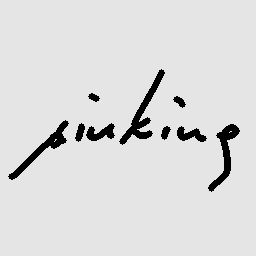
\includegraphics[scale=0.18]{../assets/background_style_transfer/spade/skeleton_gray.png}%
  %}
  %\\
 % \midrule

  Style Input &  
 % \begin{varwidth}{1in}
  \raisebox{-0.45\height}{
  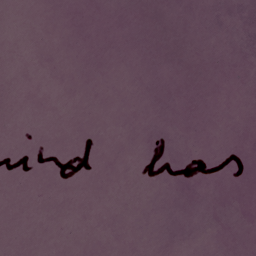
\includegraphics[scale=0.18]{../assets/background_style_transfer/spade/style/10.png}%
  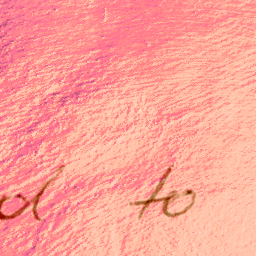
\includegraphics[scale=0.18]{../assets/background_style_transfer/spade/style/38.png}%
  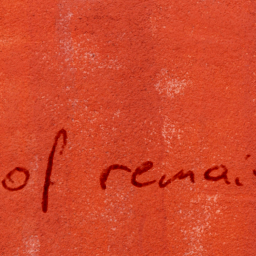
\includegraphics[scale=0.18]{../assets/background_style_transfer/spade/style/45.png}%
  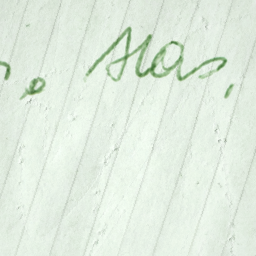
\includegraphics[scale=0.18]{../assets/background_style_transfer/spade/style/46.png}%
  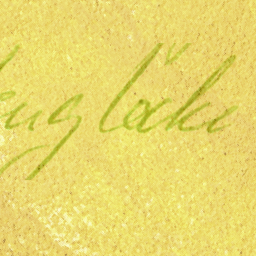
\includegraphics[scale=0.18]{../assets/background_style_transfer/spade/style/49.png}%
  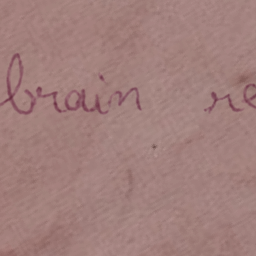
\includegraphics[scale=0.18]{../assets/background_style_transfer/spade/style/31.png}%
  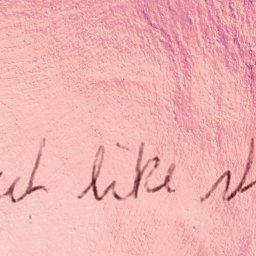
\includegraphics[scale=0.18]{../assets/background_style_transfer/spade/style/74.png}%
  %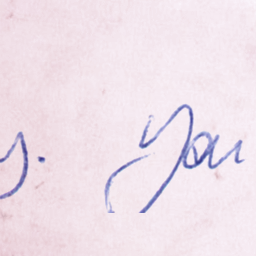
\includegraphics[scale=0.18]{../assets/background_style_transfer/spade/style/88.png}%
  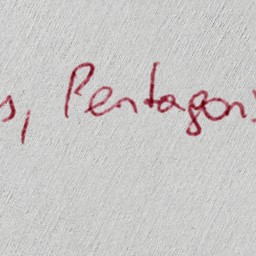
\includegraphics[scale=0.18]{../assets/background_style_transfer/spade/style/99.png}%
  %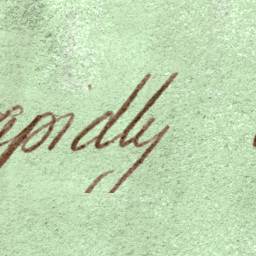
\includegraphics[scale=0.18]{../assets/background_style_transfer/spade/style/4.png}%
  %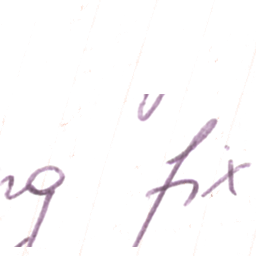
\includegraphics[scale=0.18]{../assets/background_style_transfer/spade/style/19.png}%
  %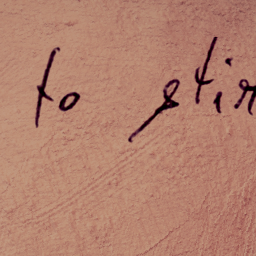
\includegraphics[scale=0.18]{../assets/background_style_transfer/spade/style/81.png}%
  %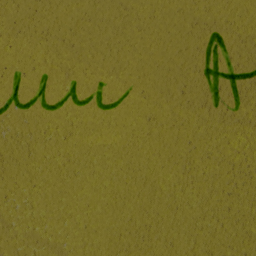
\includegraphics[scale=0.18]{../assets/background_style_transfer/spade/style/98.png}%
 % \end{varwidth}%
  }
  \\%  
  Output &
  %\begin{varwidth}{1in}
  \raisebox{-0.45\height}{
  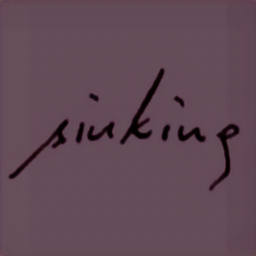
\includegraphics[scale=0.18]{../assets/background_style_transfer/spade/result_pix2pix/10.png}%
  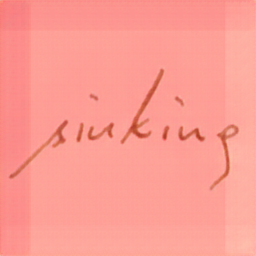
\includegraphics[scale=0.18]{../assets/background_style_transfer/spade/result_pix2pix/38.png}%
  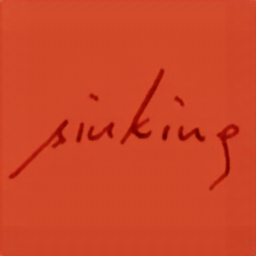
\includegraphics[scale=0.18]{../assets/background_style_transfer/spade/result_pix2pix/45.png}%
  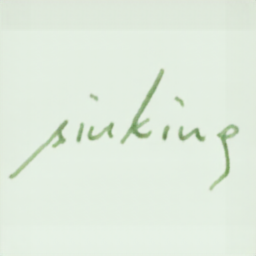
\includegraphics[scale=0.18]{../assets/background_style_transfer/spade/result_pix2pix/46.png}%
  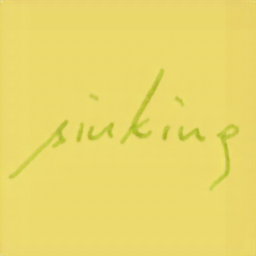
\includegraphics[scale=0.18]{../assets/background_style_transfer/spade/result_pix2pix/49.png}%
  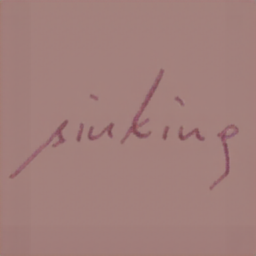
\includegraphics[scale=0.18]{../assets/background_style_transfer/spade/result_pix2pix/31.png}%
  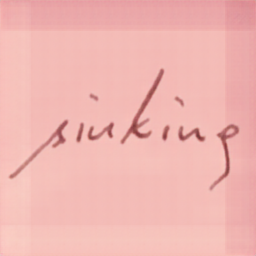
\includegraphics[scale=0.18]{../assets/background_style_transfer/spade/result_pix2pix/74.png}%
  %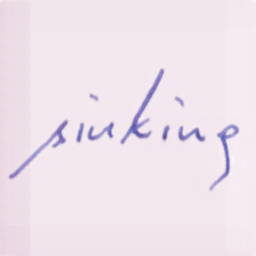
\includegraphics[scale=0.18]{../assets/background_style_transfer/spade/result_pix2pix/88.png}%
  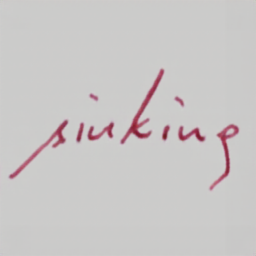
\includegraphics[scale=0.18]{../assets/background_style_transfer/spade/result_pix2pix/99.png}%
  %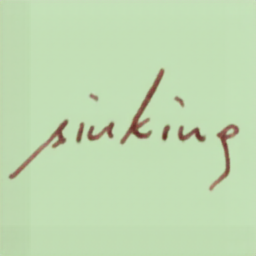
\includegraphics[scale=0.18]{../assets/background_style_transfer/spade/result_pix2pix/4.png}%
  %
\includegraphics[scale=0.18]{../assets/background_style_transfer/spade/result_pix2pix/19.png}%
  %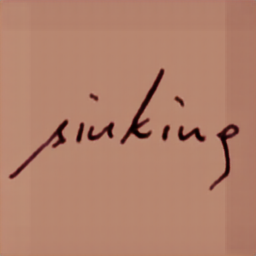
\includegraphics[scale=0.18]{../assets/background_style_transfer/spade/result_pix2pix/81.png}%
  %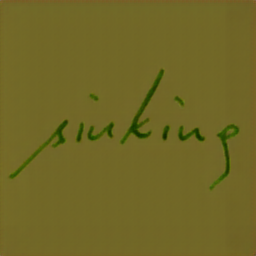
\includegraphics[scale=0.18]{../assets/background_style_transfer/spade/result_pix2pix/98.png}%
  }
  \\
  \bottomrule
  \end{tabular}
  \caption[Results of the \gls{pix2pix} based background style transfer]{Results of the \gls{pix2pix} background style transfer. While the network managed to capture both the pen and background color, its outputs are dull and lack detail.}
  \label{fig:pix2pixBackgroundResults}
\end{figure}


Nonetheless, we decided to train it anyway, to have a baseline to compare against. Surprisingly, the results were not as bad as expected and can be seen in \cref{fig:pix2pixBackgroundResults}. It successfully learned to reproduce the pen style, although with a lot less detail than when it was trained on white backgrounds. This makes sense as the style features now had to be used to represent both the foreground and the background. Additionally, as the dataset included color transformations, it had a lot more variety than the original CVL dataset. This encouraged a more aggressive generalization during the network training process, which might have contributed to the loss of detail.

While the network did learn to reproduce the color of the background, almost all of its details were lost. Similar to the pen strokes, this is most likely based on the fact that the number of style features of the network is too small.

As an implementation detail, we found that the network only converged when being trained with a fairly large batch size. To be specific, while we were able to train the network with 16 samples per batch, training attempts with a batch size of one or two were dominated by artifacts. The same is to be said about the image synthesis, which created large artifacts if run with other batch sizes than the network was trained on. This is most likely caused by the batch normalization stages, though further studies are required to gain a deeper understanding of that phenomenon.

\subsection{Modifications to the network}
In an attempt to improve the results, we decided to reconfigure the network to be more suited for the current task. As the background requires a lot more global information than the pen strokes, we increased the depth and the feature count of both the decoder and style extractor. The encoder still only encounters skeleton images, and therefore we left the encoder at 4 layers, with skip connections to the 4 uppermost layers of the decoder.

To give the network more control over the style input, we decided to merge the style information into all layers of the decoder network, not just the innermost layer. This should give the network the power to decide at what depth it wants to use which style information.

Sadly, we weren't able to successfully train the network, as we didn't find a converging configuration. All our attempts were dominated by major artifacts without any sign of improvement. As the reconfiguration increased the size of the network, we were forced to reduce the number of samples per batch again, which might be partially responsible for our results. Nonetheless, further research might solve this problem, which makes this approach a potential candidate for future work.




\section{SPADE}\label{section:backgroundTransferSpade}


\begin{figure}
  \centering
  \begin{tabular}{lc}
  \toprule
  
  %Skeleton &
  %\raisebox{-0.45\height}{
  %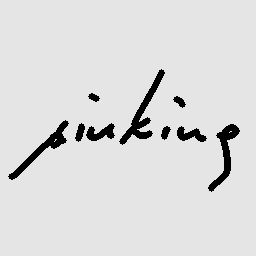
\includegraphics[scale=0.18]{../assets/background_style_transfer/spade/skeleton_gray.png}%
  %}
  %\\
 % \midrule

  Style Input &  
 % \begin{varwidth}{1in}
  \raisebox{-0.45\height}{
  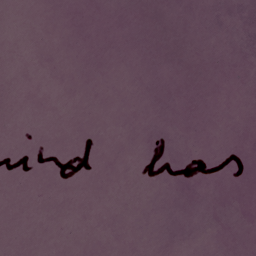
\includegraphics[scale=0.18]{../assets/background_style_transfer/spade/style/10.png}%
  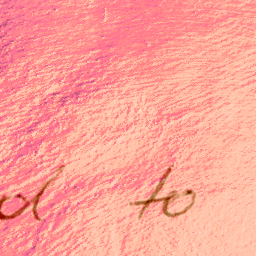
\includegraphics[scale=0.18]{../assets/background_style_transfer/spade/style/38.png}%
  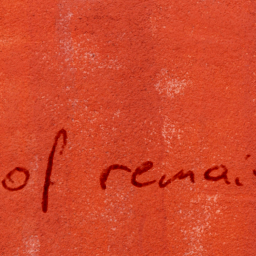
\includegraphics[scale=0.18]{../assets/background_style_transfer/spade/style/45.png}%
  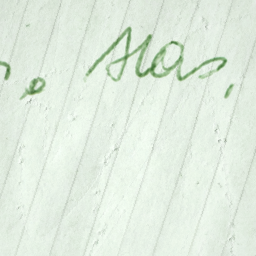
\includegraphics[scale=0.18]{../assets/background_style_transfer/spade/style/46.png}%
  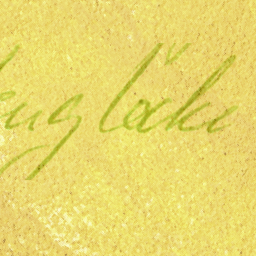
\includegraphics[scale=0.18]{../assets/background_style_transfer/spade/style/49.png}%
  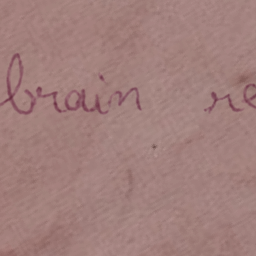
\includegraphics[scale=0.18]{../assets/background_style_transfer/spade/style/31.png}%
  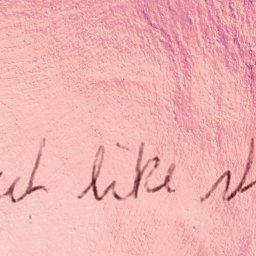
\includegraphics[scale=0.18]{../assets/background_style_transfer/spade/style/74.png}%
  %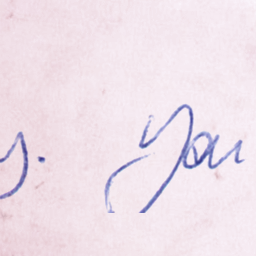
\includegraphics[scale=0.18]{../assets/background_style_transfer/spade/style/88.png}%
  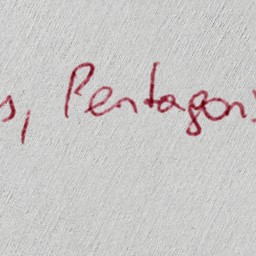
\includegraphics[scale=0.18]{../assets/background_style_transfer/spade/style/99.png}%
  %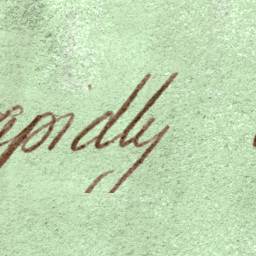
\includegraphics[scale=0.18]{../assets/background_style_transfer/spade/style/4.png}%
  %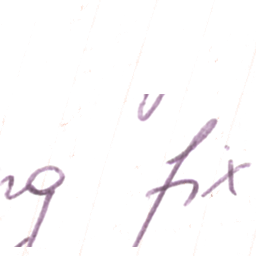
\includegraphics[scale=0.18]{../assets/background_style_transfer/spade/style/19.png}%
  %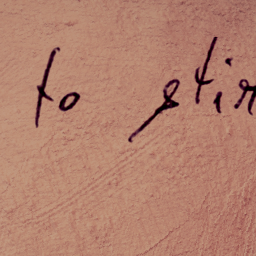
\includegraphics[scale=0.18]{../assets/background_style_transfer/spade/style/81.png}%
  %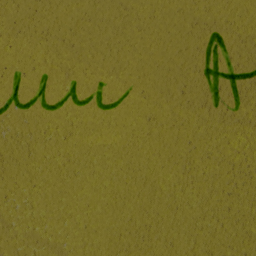
\includegraphics[scale=0.18]{../assets/background_style_transfer/spade/style/98.png}%
 % \end{varwidth}%
  }
  \\%  
  Output &
  %\begin{varwidth}{1in}
  \raisebox{-0.45\height}{
  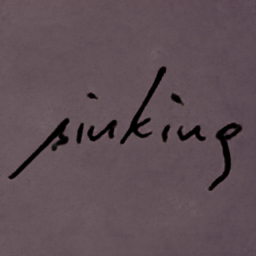
\includegraphics[scale=0.18]{../assets/background_style_transfer/spade/result/10.png}%
  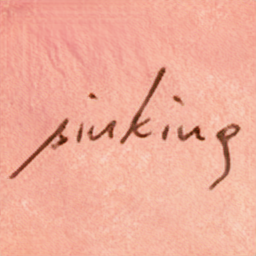
\includegraphics[scale=0.18]{../assets/background_style_transfer/spade/result/38.png}%
  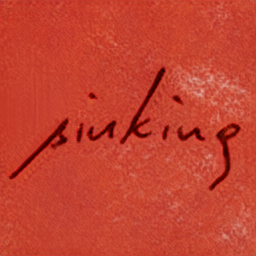
\includegraphics[scale=0.18]{../assets/background_style_transfer/spade/result/45.png}%
  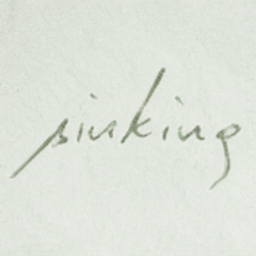
\includegraphics[scale=0.18]{../assets/background_style_transfer/spade/result/46.png}%
  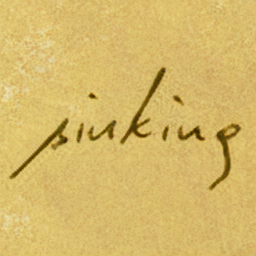
\includegraphics[scale=0.18]{../assets/background_style_transfer/spade/result/49.png}%
  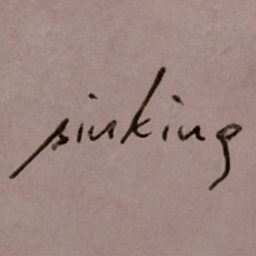
\includegraphics[scale=0.18]{../assets/background_style_transfer/spade/result/31.png}%
  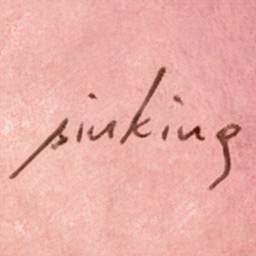
\includegraphics[scale=0.18]{../assets/background_style_transfer/spade/result/74.png}%
  %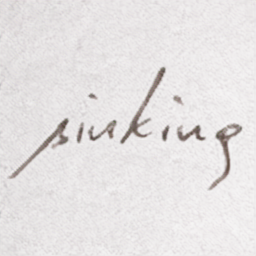
\includegraphics[scale=0.18]{../assets/background_style_transfer/spade/result/88.png}%
  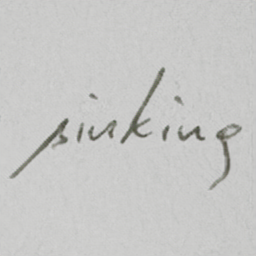
\includegraphics[scale=0.18]{../assets/background_style_transfer/spade/result/99.png}%
  %\includegraphics[scale=0.18]{../assets/background_style_transfer/spade/result/4.png}%
  %\includegraphics[scale=0.18]{../assets/background_style_transfer/spade/result/19.png}%
  %\includegraphics[scale=0.18]{../assets/background_style_transfer/spade/result/81.png}%
  %\includegraphics[scale=0.18]{../assets/background_style_transfer/spade/result/98.png}%
  }
  \\
  \bottomrule
  \end{tabular}
  \caption[Results of the \gls{spade} network]{Results of the \gls{spade} network. While the network was able to synthesize quite realistic backgrounds, it never learned to match the original text color.}
  \label{fig:spadeResults}
\end{figure}


At the time of writing, NVidia just released the \gls{spade} network~\cite{spade}, which is built to generate photorealistic images from a style reference photo and a segmentation map. Contrary to our attempt, the \gls{spade} network does not add the style information by concatenation with the feature vectors but instead uses it to control the normalization parameters of the network, which seems to give the network the ability to learn the styles of the different objects separately and with more detail.

As the network internally downsamples the segmentation map multiple times, our skeleton images are incompatible with it, as all strokes with a diameter of a single pixel would disappear during downsampling. To solve that problem, we applied morphologic dilation to the skeleton images until the lines were thick enough to be picked up by the network. To be specific, we used a circular dilation with a radius of 6 pixels.

\subsection{Results}



\gls{spade} was able to understand and recreate the backgrounds of the images better than our modified \gls{pix2pix}, as seen in \cref{fig:spadeResults}. It managed to include some detail, especially if the background included some degree of noise. Nonetheless, it wasn't able to reproduce high-frequency details, like thin lines, which are quite common on paper. This is similar to the problems we encountered earlier and is a more general problem with \glspl{cnn} than with this specific network.

Sadly, we never got it to converge on the color of the pen strokes. This might be based on the fact that the pen strokes only take up a very small portion of the image compared to the background, reducing the priority of the pen strokes far enough that they don't get included in the style information. This could possibly be mitigated by modifying the loss function and should be researched further in future work.


\section{Multi Step Approach}
As the previous attempts failed, we decided to split the task into sub-problems that are either already solved, or relatively simple.
In theory, if we managed to extract the foreground from the background, we could apply the pen style transfer algorithm of \cref{chapter:imageStyleTransfer} to the foreground and then merge it back into the background.


\begin{figure}
  \centering
  \includegraphics[width=0.95\textwidth]{../assets/background_style_transfer/pipeline/pipeline.pdf}
  \caption[The multi-step approach for the background style transfer]{The multi-step approach for the background style transfer. First, the foreground of the input image is extracted. The extracted foreground image is then removed from the background, leaving holes behind. Next, the background is reconstructed with a hole inpainting algorithm. In the meantime, the extracted foreground is passed into the style transfer pipeline of the previous chapters to create the synthetic text image. Finally, the foreground and the background are merged back together.}
  \label{fig:backgroundPipeline}
\end{figure}


We therefore propose a pipeline with the following steps, as seen in \cref{fig:backgroundPipeline}:

\begin{enumerate}[topsep=0pt,itemsep=-1ex,partopsep=1ex,parsep=1ex]
\item Extracting the foreground, the actual handwriting, from the input image
\item Creating a foreground mask from the foreground image by thresholding and dilation
\item Removing the masked regions from the background image, followed by an inpainting of the remaining holes
\item Running the existing style transfer pipeline on the foreground image
\item Merging the result of the style transfer pipeline back into the background image
\end{enumerate}

\textbf{Foreground extraction}. Training a foreground extractor was straight forward, as this problem is similar to the skeletonization problem described in \cref{chapter:skeletonization}, for which we achieved satisfying results by utilizing the \gls{pix2pix} network. The difference was that we needed a new training dataset, which we were able to generate by storing both the foregrounds, backgrounds and merged images separately during the generation of the dataset of \cref{section:backgroundDataset}.

\textbf{Hole filling}. With the foreground extracted, we were able to create a binary mask and remove it from the background, leaving holes. Filling the holes back in was a non-trivial task, and we decided to utilize NVidia's hole filling network~\cite{nvidiaInpaint}, which is based on partial convolutions, a concept also developed by NVidia.~\cite{nvidiaPconv} As they did not publish the code of their image inpainting demo, we decided to implement it ourselves~\cite{infillOurs}.
This gave us a background that is not just style transferred from the original image, but mostly identical.

\textbf{Merging}. Merging the result of the network back into the images was also a non-trivial step. To get a result that looks identical to the original image, it was important that the merging was equivalent to undoing the foreground extraction step. As the foreground extraction was trained on a synthetic dataset, the merging operation had to be identical to the one used during dataset generation. While most certainly more sophisticated algorithms exist, in our case we merged with a simple inverted addition:

\begin{equation}
c_{out} = 255 - ((255 - c_{foreground}) + (255 - c_{background}))
\end{equation}
\begin{equation}
c_{out} = c_{foreground} + c_{background} - 255
\end{equation}

As the output is supposed to be a color value between $0$ and $255$, we then clipped the result into the desired range.

\subsection{Results}

While our approach is promising, we cannot draw a definite conclusion at this point. Multiple issues need to be resolved before a real evaluation can take place.

For one, the style transfer pipeline of the previous chapters was only trained on CVL-like images so far and is therefore not capable of generating all the possible styles we have in the background transfer dataset. This is caused by the random color transformations we used during dataset generation and would require a re-training of the pen style transfer stage.


Further, the foreground extraction we trained did fairly well on our synthetic dataset, but performed poorly on real-world data, as seen in \cref{fig:foregroundExtractionFail}. As the network itself is most certainly capable of solving this task properly, the reason for the poor behavior is most likely the dataset itself, and finding better alternatives for the dataset generation would be one of the first improvements for future work.

\begin{figure}
  \centering
  \subfloat[Foreground extraction from synthetic data]{
  	\hspace{0.06\textwidth}
  	\adjustbox{cframe=gray}{%
  	\includegraphics[width=0.16\textwidth]{../assets/background_style_transfer/pipeline/input_with_background.png}%
  	\includegraphics[width=0.16\textwidth]{../assets/background_style_transfer/pipeline/foreground_extracted.png}%
  	}
  	\hspace{0.06\textwidth}
  }
  \subfloat[Foreground extraction from real data]{
  	\hspace{0.06\textwidth}
    \adjustbox{cframe=gray}{%
  	\includegraphics[width=0.16\textwidth]{../assets/background_style_transfer/pipeline/handschrift_boerns_cropped.png}%
  	\includegraphics[width=0.16\textwidth]{../assets/background_style_transfer/pipeline/handschrift_boerns_cropped_foreground.png}%
  	}
  	\hspace{0.06\textwidth}
  }
  \caption[Problems with the foreground extraction on real data]{Problems with the foreground extraction on real data. While the network performs flawlessly on the test dataset, it seems to struggle with real world data. This indicates that some crucial detail of our dataset is different from real world data.}
  \label{fig:foregroundExtractionFail}
\end{figure}


